\documentclass[11pt, a4paper]{article}
\usepackage{graphicx, fullpage, hyperref, listings}
\usepackage{appendix, pdfpages, color}
\usepackage{indentfirst} %段首空两格 棒
\usepackage{chngpage} 
\usepackage{tocloft}            % This squashes the Table of Contents a bit
\usepackage{pdfpages}
\usepackage{multirow}
\usepackage{amsmath}
\usepackage{framed}


\setlength\cftbeforesecskip{3pt}
\renewcommand{\contentsname}{\centerline{\textbf{Content}}}
\graphicspath{{images/}}

\usepackage{multicol}

\usepackage{graphicx}
\usepackage{epstopdf}
\hypersetup{CJKbookmarks,%
	bookmarksnumbered,%
	colorlinks,%
	linkcolor=black,%
	citecolor=black,%
	plainpages=false,%
	pdfstartview=FitH}

%%%%%%%代码语法高亮设置

\usepackage{color}

\definecolor{pblue}{rgb}{0.13,0.13,1}
\definecolor{pgreen}{rgb}{0,0.5,0}
\definecolor{pred}{rgb}{0.9,0,0}
\definecolor{pgrey}{rgb}{0.46,0.45,0.48}

\usepackage{listings}
\lstset{
	language=Java,
	showspaces=false,
	showtabs=false,
	%%%%%
	frame = single,
	stepnumber = 2,  
	numbersep = 4pt, 
	 numbers=left,
	%breakatwhitespace=false, 
	tabsize=2,  
	%%%%%
	breaklines=true,
	showstringspaces=false,
    breakatwhitespace=false, 
	commentstyle=\color{pgreen},
	keywordstyle=\color{pblue},
	stringstyle=\color{pred},
	basicstyle=\ttfamily,
	%moredelim=[il][\textcolor{pgrey}]{$$},
	%moredelim=[is][\textcolor{pgrey}]{\%\%}{\%\%},
}


%%%%%%%%代码语法高亮设置

\definecolor{MyLightYellow}{cmyk}{0,0.,0.2,0} 

\setlength{\parskip}{4pt}        % sets spacing between paragraphs
\interfootnotelinepenalty=500    % this prevents footnotes breaking across pages

\title{
\includegraphics[width=0.45\textwidth]{wpi2}
        \\CS 534 Artificial Intelligence \\ Assignment 2 }          % <<<<<<<<< change the title as appropriate
\author{Group 10 }                    % <<<<<<<<< module code

\begin{document}
\begin{titlepage}
	
%\date{\today}
\maketitle
\addtocontents{toc}{\protect\thispagestyle{empty}} % because we don't want a page number on the title page
% Thanks to Huang Shanyue for suggesting this 

\begin{center}
Group Member
\end{center}

\begin{table}[htbp] 
\begin{center}
\begin{tabular}{l l l} 
	 
	 Yixuan & Jiao  &   yjiao@wpi.edu \\
     Yinkai & Ma  &   yma7@wpi.edu \\
     Jiaming & Nie  &  jnie@wpi.edu \\
     Pinyi & Xiao  &  pxiao@wpi.edu \\
\end{tabular}
\end{center}
\end{table}



%\date{\today}
\thispagestyle{empty}  %去除首页页码

\end{titlepage}

%\tableofcontents
%\listoffigures

%\newpage



%\tableofcontents

%\listoffigures
%\listoftables
%\lstlistoflistings        


%\newpage

\section{Gibbs Sampling}

\subsection{Procedures}

\subsubsection{Load The Data}

The data of the Bayesian network is stored on the excel, so when load the excel, this project could get the data we need in the next step. The format of the input is as following:

gibbs price schools=good location=ugly -u 10000 -d 0

The price is the query node, and the schools and location are the evidence nodes. 10000 means the iteration, 0 means discard 0.
In this step, this project could get the request of the Gibbs sampling.

\subsection{Gibbs Sampling}

In order to do the Gibbs sampling, we need to know the information from the excel and input. For each iteration, we need to update the state of every node and store the state after update. After the iteration, the probability could be computed by the stored state.


The sequence of updating is shown below:
['amenities', 'neighborhood', 'children', 'age', 'location', 'size', 'schools', 'price']

\subsubsection{Operation of Gibbs sampling}

In order to do the gibbs sampling, we need to know the information from the excel and input. For each iteration, we need to update the state of every node and store the state after the update. After the iteration, the probability could be computed by the stored state.


The sequence of updating is shown below:
['amenities', 'neighborhood', 'children', 'age', 'location', 'size', 'schools', 'price']

\paragraph{Set the evidence}

For no update is made to evidence nodes, we need an approach to distinguish them from the rest nodes.We generate a list to store the information of evidence nodes. 


\section{Kalman Filter}



\subsection{Model Hypothesis}
The transition model is constructed using the GDP and the gdp growth rate from 1970 to 2017, data source is from world bank website~\cite{ref:source1}. Unit is trillion dollar.

There are 2 sensor models, in the first model our group use the Export and Import data from 1970 to 2017~\cite{ref:source2}, the unit is value in million dollars, to measure the GDP only, which is use the 2 sensors to measure the GDP. 

The second model is use 3 sensors, the 2 sensors are still import and export, the additional sensor is the employment rate~\cite{ref:source3}, to measure the GDP growth rate. The data source is from Office of Management and Budget. 

\subsubsection{Kalman Filter Network}

\begin{figure}[htbp]
	
	\centering 
	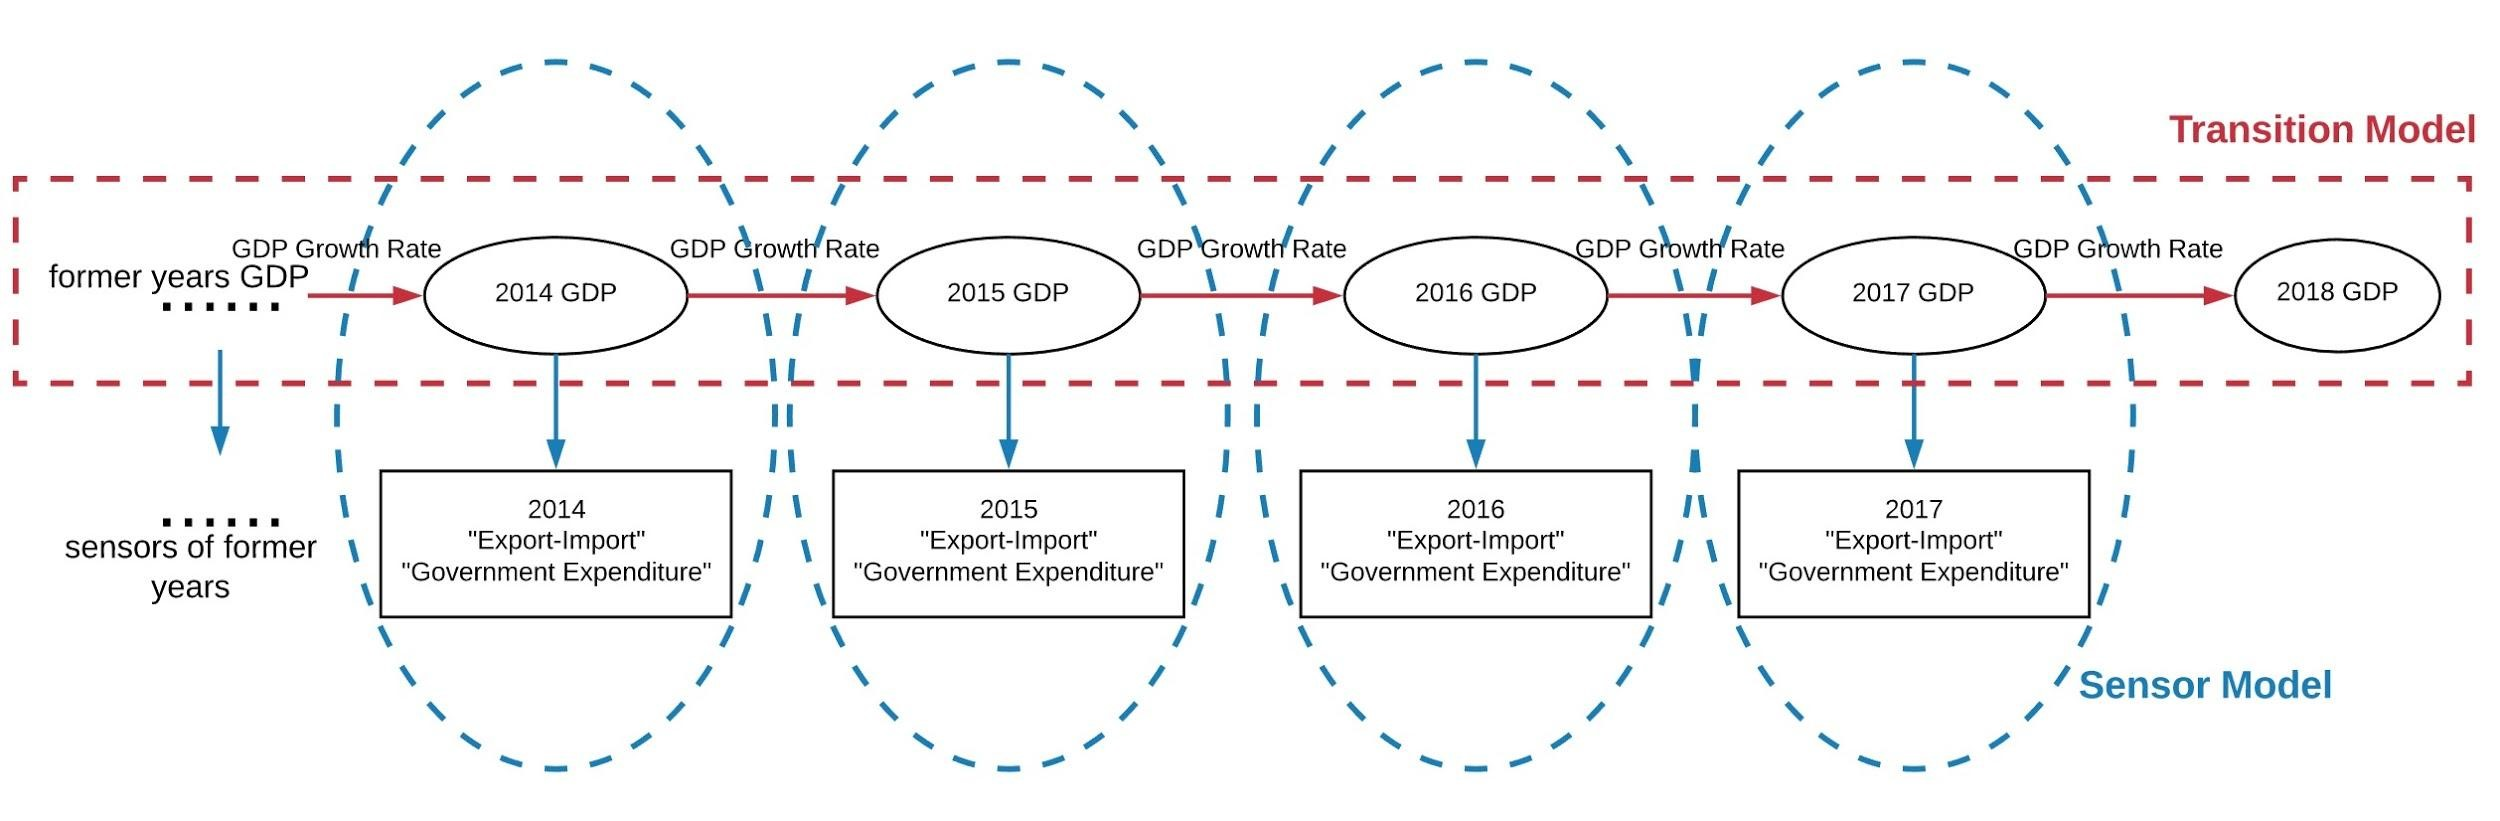
\includegraphics[width=10cm]{graph}
	
	\caption{Kalman Filter Network}
	\label{fig:network}
	
\end{figure}


\subsection{Methodology}

\subsubsection{Kalman Filter Graph Model and Equations}
The graph model of the Kalman filter is on the following:



The parameters of the Kalman filter and their equations are on the following~\cite{ref:kf}.

For Kalman filter, its parameters are listed in the table~\ref{tab:kf_meaning}:

\begin{table}[htbp] 
	\begin{center}
		\caption{Kalman Filter Parameters Notation}
		\begin{tabular}{|l|p{400pt}|} \hline
			Parameter & Notation \\ \hline
			${x_t}$ & The state vector containing the terms of interest for the system (e.g., position, velocity, heading) at a time 
			\\ \hline
			${F_t}$ & The state transition matrix which applies the effect of each system state at time \textit{t}. (e.g., the position and velocity at time t-1 both affect the position at time t) \\ \hline
			${w_t}$ & the vector which contains the noise for each parameter in the state vector ${x_t}$. A zero mean multivariate Gaussian distribution with covariance matrix ${Q_t}$ is used to describe the process noise vector. \\ \hline
			${z_t}$ & The measurements vector. \\ \hline
			${H_t}$ & the transformation matrix which can interpret the state vector ${x_t}$ into measurement domain of ${z_t}$. \\ \hline
			${v_t}$ &  the measurement noise vector for each observed value in the measurement vector ${z_t}$. The model that to establish the measurement noise is also drawn from a zero mean multivariate normal distribution with covariance matrix ${R_t}$. \\ \hline
			${R_t}$ & The covariance matrix for the observation noise. \\ \hline
			${Q_t}$ & The covariance matrix for the process noise. \\ \hline
			
		\end{tabular}
		
		\label{tab:kf_meaning}
	\end{center}
\end{table}

In the Kalman filter, the state matrix can be described as~\ref{eq:1}, which is transition model.

\begin{equation}
x_{t} = F_{t}x_{t-1} + w_t 
\end{equation}\label{eq:1}

At the time $t$ an observation $z_t$ of the true state $x_t$ is made according to~\ref{eq:2}, which represents the observation model.

\begin{equation}
	z_t = H_tx_t + v_t
\end{equation}\label{eq:2}

The state of the filter is represented by 2 variables:

\begin{table}[htbp]
 \begin{center}
 	\begin{tabular}{l|l} \hline
 		$\widehat{x}_{t|t} $ & a posterior state estimate given the observations up to $t$ \\ \hline
 		$\widehat{P}_{t|t} $ & a posterior error covariance estimate given the observations up to $t$ \\ \hline
 	\end{tabular}
 
\end{center}
\end{table}

The predict process of the Kalman filter can be described using equation~\ref{eq:3} and~\ref{eq:4}. 

\begin{equation}
	\widehat{t}_{t|t-1} = F_t\widehat{t}_{t-1|t-1} 
\end{equation}\label{eq:3}

\begin{equation}
P_{t|t-1} = F_tP_{t-1|t-1}F_{t}^T + Q_{t}
\end{equation}\label{eq:4}

The update process of the Kalman filter is on the following, $\widetilde{y}_{t}$ is the residual covariance, $K_{t}$ is the Kalman gain matrix:

\begin{equation}
\widetilde{y}_{t} = z_t - H_t\widehat{x}_{t|t-1} \end{equation}

\begin{equation}
S_t = R_t + H_tP_{t|t-1}H_{t}^T \end{equation}

\begin{equation}
K_t = P_{t|t-1}H_{t}^{T}S_{t}^{-1} \end{equation}

\begin{equation}
\widehat{x}_{t|t} = \widehat{x}_{t|t-1}+K_t\widetilde{y}_{t} \end{equation}

\begin{equation}
P_{t|t} = (I - K_tH_t)P_{t|t-1}{(I-K_tH_T)}^{T} + K_t \end{equation}

\begin{equation}
\widetilde{y}_{t|t} = z_t - H_t\widehat{x}_{t|t}
\end{equation}

\subsubsection{Transition Model}

In the transition model, a state is defined by the GDP and GDP growth rate. For a state $x_k$, $x_k = \begin{bmatrix} x_g \\ x_{gr}  \end{bmatrix}$. $x_g$ represents the state of the GDP and $x_{gr}$ represents the state of the GDP growth rate. The transition matrix $F_t$ is calculated based on the matrix $Q_t$.

In the transition model, our group used the linear fitting to estimate the relationship between the GDP and GDP growth rate on the condition that the GDP growth rate is set to constant. 

The estimated linear relationship is on the following equation~\ref{eq:5}:

\begin{equation}
y_{GDP} = -0.687\times x_{growth rate} + 11.3324
\label{eq:5}
\end{equation}

According to the linear relationship, the transition matrix $F$ is $F = \begin{bmatrix} 1 & -0.687 \\ 0 & 1  \end{bmatrix}$

In the transition model, assume the the Pearson's coefficient $\rho$ between the GDP growth rate and the GDP is 0, which is that the variation between GDP $x_g$ and GDP growth rate $x_{gr}$ does not have any dependency. Then the process noise matrix $Q$ is 
\begin{center}
$Q = \begin{bmatrix} var(x_g) & 0 \\ 0 & var(x_{gr})  \end{bmatrix}$ 
\end{center}

Then the matrix $w_k$ is $w_k = \mathcal{N}(0,Q)$.


\subsubsection{Sensor Model}

Export and import data will be 2 sensors to measure the GDP data and the employment rate will be the sensor to measure the GDP growth rate as the extra credit part. 

\paragraph{Sensor Model for GDP only}

In the sensor model for GDP purely, the GDP is measured by the Export and Import, construct the linear polyfit model for the GDP using export and import, 

the equation is on the following equation~\ref{eq:6} and~\ref{eq:7}:

\begin{equation}
y_{GDP} = 0.4943\times x_1 + 5.1524 (x_1:Export)
\label{eq:6}
\end{equation}

\begin{equation}
y_{GDP} = 0.3435\times x_2 + 5.1855 (x_2:Import)
\label{eq:7}
\end{equation}


Then the observe matrix $H$ is $H = \begin{bmatrix} 0.4943 & 0 \\ 0.3435 & 0   \end{bmatrix}$


Assume the export and import data does not have any dependency, then the noise matrix $R$ is:

\begin{center}
	$R = \begin{bmatrix} var(Export) & 0  \\ 0 & var(Import)  \end{bmatrix}$
\end{center}

Then the matrix $v_k$ is $v_k = \mathcal{N}(0,R)$

\paragraph{Sensor Model for GDP and GDP growth Rate}

In the sensor model which already has 2 sensors for the GDP, add 1 sensor for the GDP growth rate. 

The sensor for the GDP growth rate $y$ adopts the employment rate $x$,the linear fitting result is illustrated in equation~\ref{eq:8}:

\begin{equation}
y = -0.074\times x + 7.7465 
\label{eq:8}
\end{equation}

Then the observe matrix $H$ is $H$ is $H = \begin{bmatrix} 0.4943 & 0 \\ 0.3435 & 0 \\ 0 & -0.074  \end{bmatrix}$


Assume the export data, import data and the employment rate does not have any dependency, then the noise matrix $R$ is:

\begin{center}
	$R = \begin{bmatrix} var(Export) & 0 & 0 \\ 0 & var(Import) & 0 \\ 0 & 0 & var(employRate)  \end{bmatrix}$
\end{center}

Then the matrix $v_k$ is $v_k = \mathcal{N}(0,R)$

\subsection{Results}

\subsubsection{Kalman Estimate Result: Sensor for GDP only (2 Sensors)}


\paragraph{Probability Distribution}

The probability distribution for GDP is illustrated in~\ref{fig:pd_1}.

\begin{figure}[htbp]
	
	\centering 
	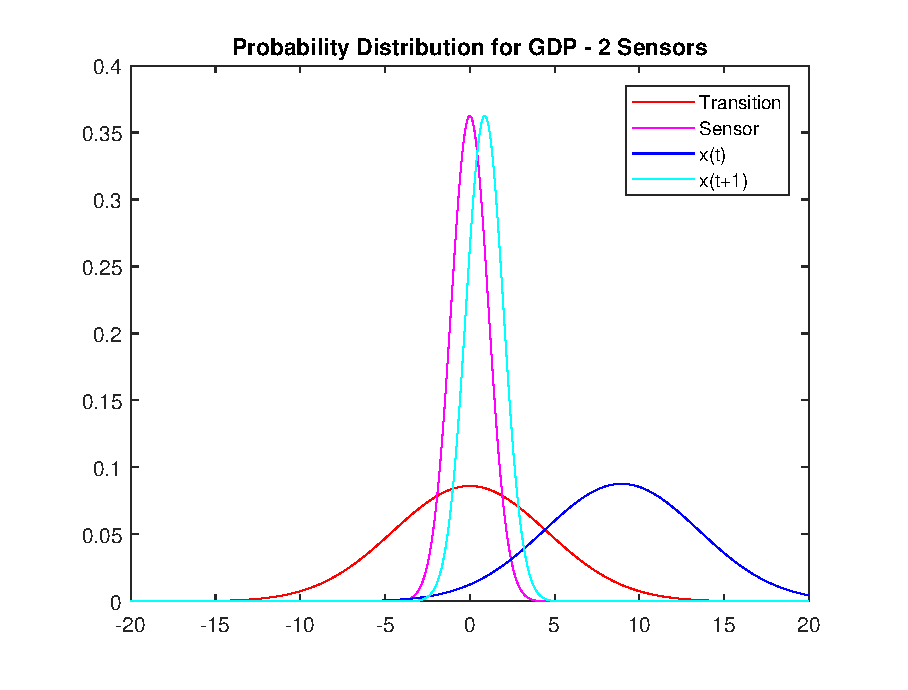
\includegraphics[width=10cm]{pd_1}
	
	\caption{2-Sensor Model GDP Probability Distribution}
	\label{fig:pd_1}
	
\end{figure}

The probability distribution for GDP growth rate is illustrated in~\ref{fig:pd_2}.

\begin{figure}[htbp]
	
	\centering 
	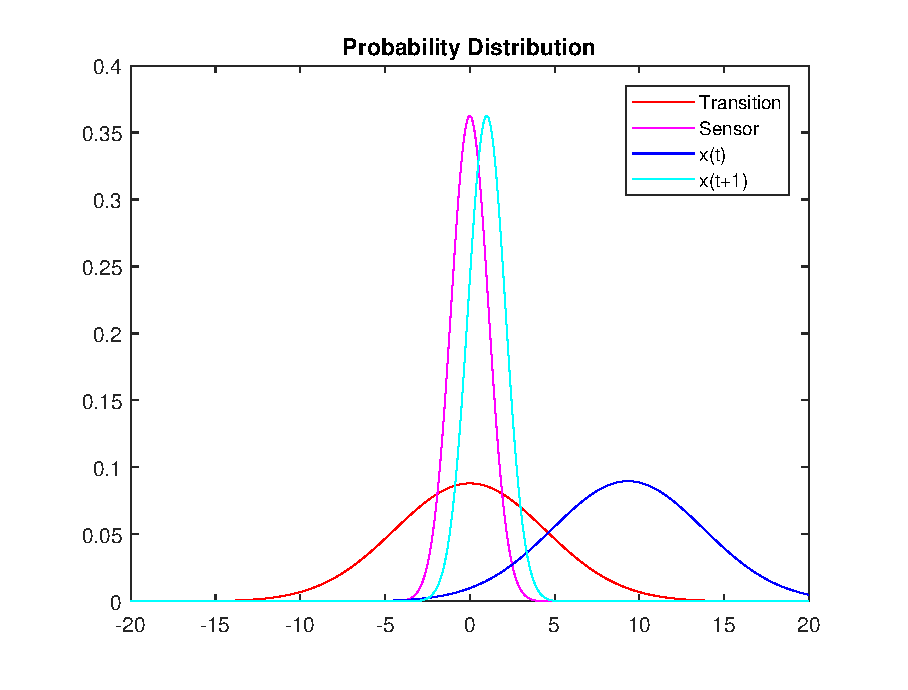
\includegraphics[width=10cm]{pd_2}
	
	\caption{2-Sensor Model GDP Growth Rate Probability Distribution}
	\label{fig:pd_2}
	
\end{figure}



\paragraph{The Estimate Result Under Transition Model Only}

\subparagraph{GDP Estimate}

The estimate result of GDP under the transition model only is illustrated in figure~\ref{fig:kf1}.

 \begin{figure}[htbp]
	
	\centering 
	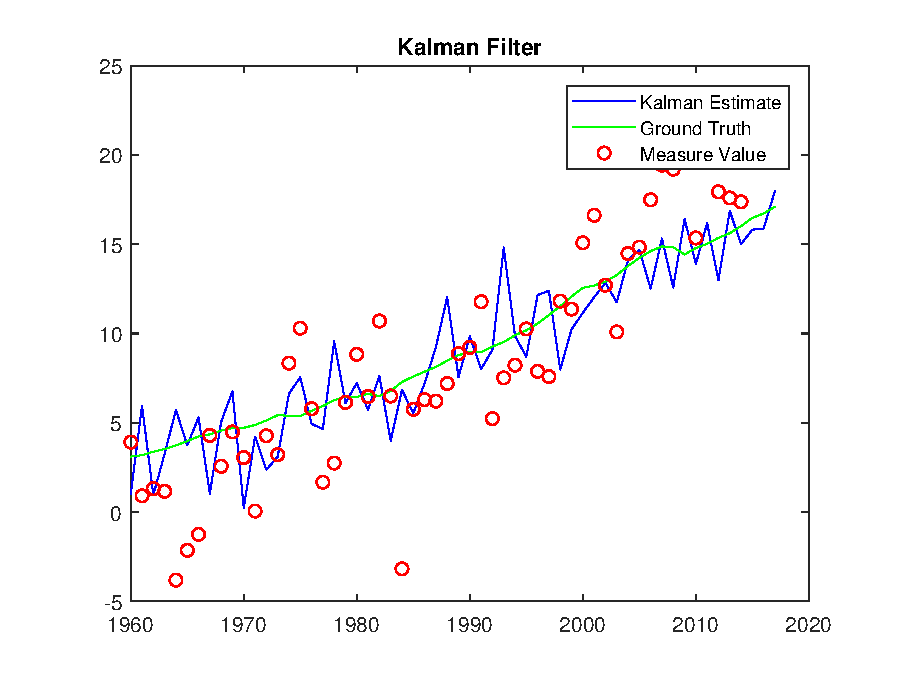
\includegraphics[width=10cm]{kf_1_1}
	
	\caption{Kalman Estimate for GDP (Transition Model Only)}
	\label{fig:kf1}
	
\end{figure}




\subparagraph{GDP Growth Rate Estimate}

The estimate result of GDP growth rate under the transition model only is illustrated in figure~\ref{fig:kf2}.

\begin{figure}[htbp]
	
	\centering 
	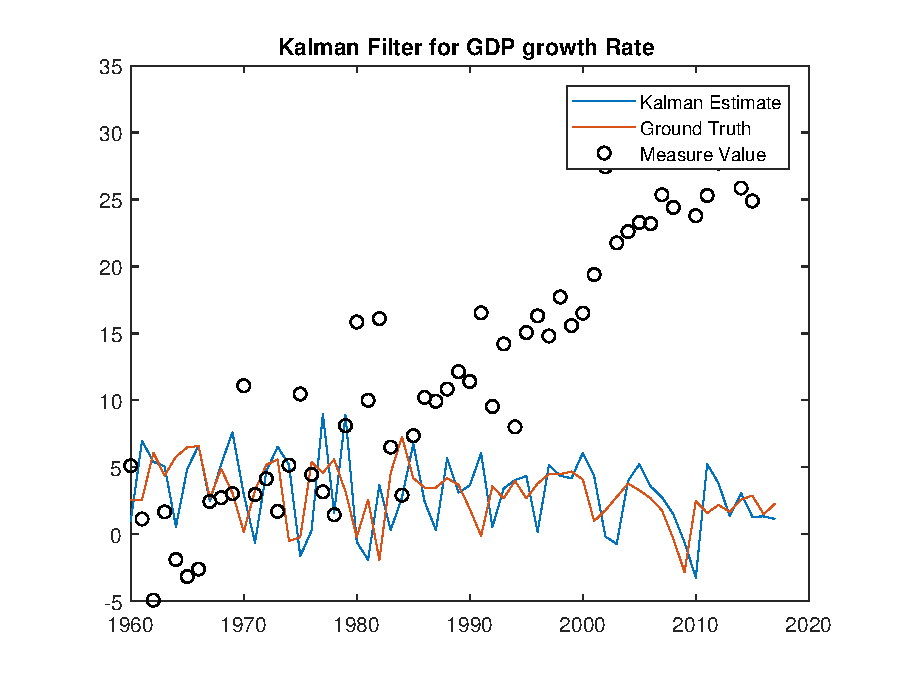
\includegraphics[width=10cm]{kf_1_2}
	
	\caption{Kalman Estimate for GDP growth rate (Transition Model Only)}
	\label{fig:kf2}
	
\end{figure}

\paragraph{Estimate Result for Transition and Sensor Model}

\subparagraph{GDP Estimate}

The estimate result of GDP under the complete model is illustrated in figure~\ref{fig:kf3}.

\begin{figure}[htbp]
	
	\centering 
	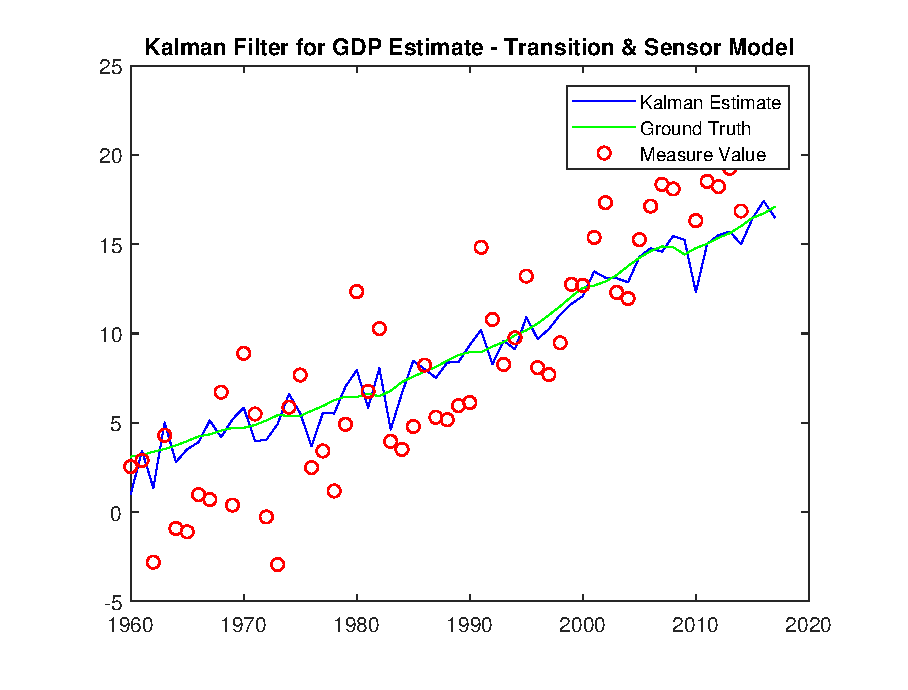
\includegraphics[width=10cm]{kf_1_3}
	
	\caption{Kalman Estimate for GDP (Complete Model)}
	\label{fig:kf3}
	
\end{figure}

\subparagraph{GDP Growth Estimate}

The estimate result of GDP under the complete model is illustrated in figure~\ref{fig:kf4}.

\begin{figure}[htbp]
	
	\centering 
	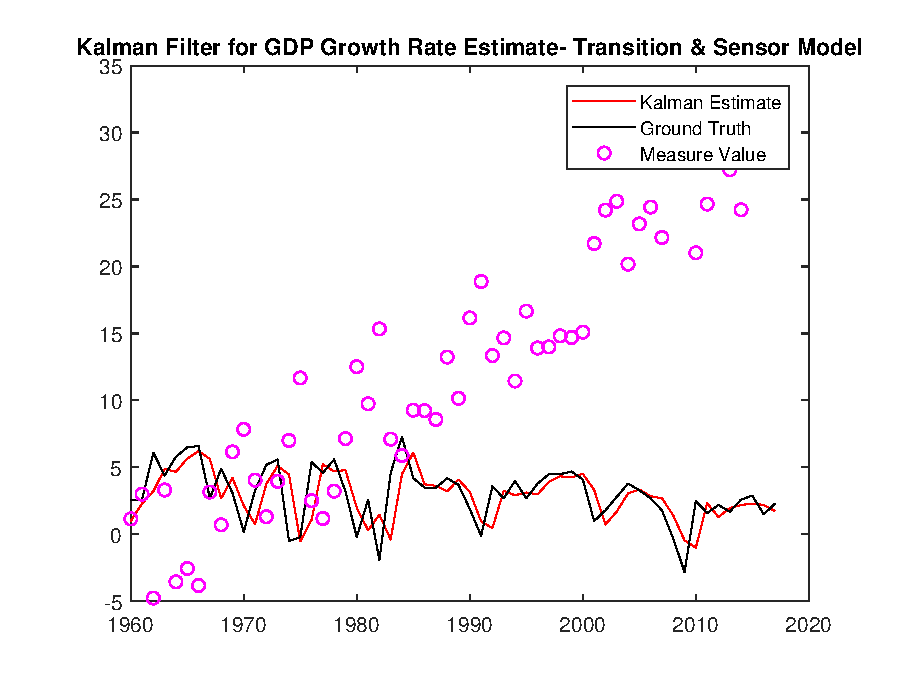
\includegraphics[width=10cm]{kf_1_4}
	
	\caption{Kalman Estimate for GDP Growth Rate (Complete Model)}
	\label{fig:kf4}
	
\end{figure}


\subsubsection{Extra Part: Additional Sensor for GDP growth rate }

\paragraph{Probability Distribution}

The probability distribution for GDP is illustrated in~\ref{fig:pd_3}.

\begin{figure}[htbp]
	
	\centering 
	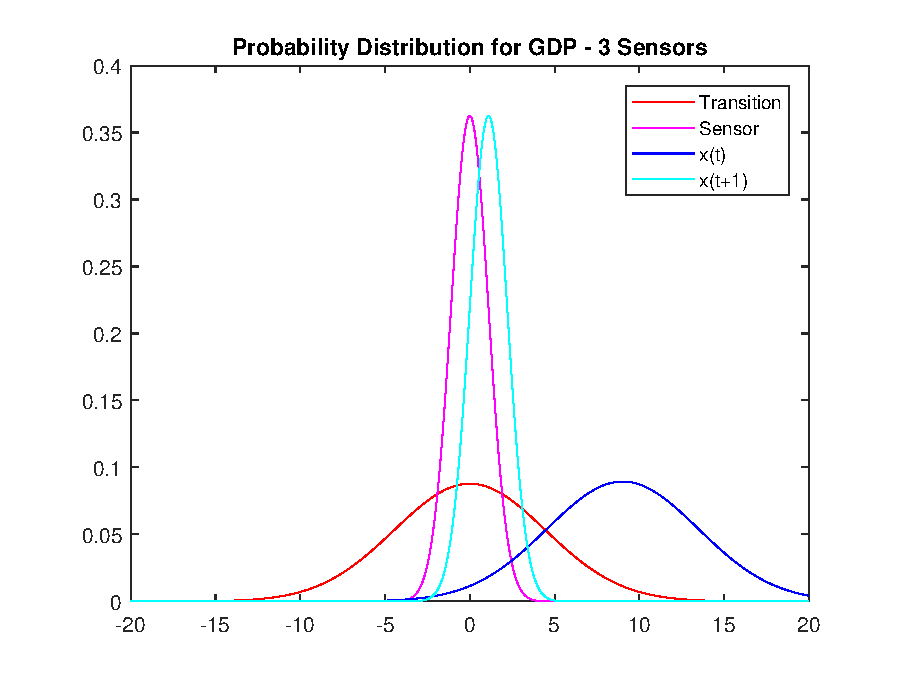
\includegraphics[width=10cm]{pd_3}
	
	\caption{3-Sensor Model GDP Probability Distribution}
	\label{fig:pd_3}
	
\end{figure}

The probability distribution for GDP growth rate is illustrated in~\ref{fig:pd_4}.

\begin{figure}[htbp]
	
	\centering 
	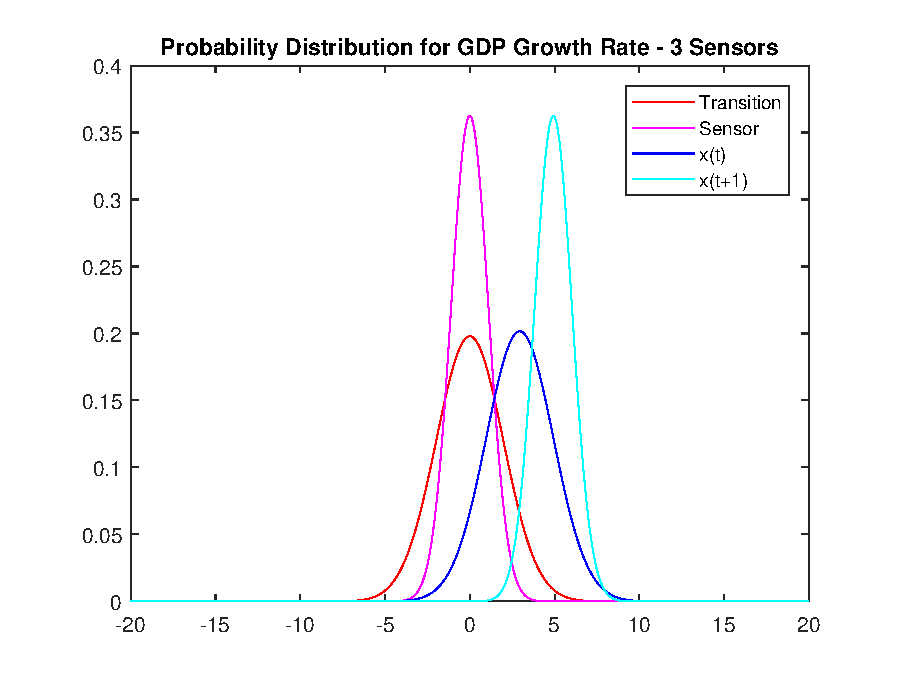
\includegraphics[width=10cm]{pd_4}
	
	\caption{3-Sensor Model GDP Growth Rate Probability Distribution}
	\label{fig:pd_4}
	
\end{figure}


\paragraph{Estimate Result for Transition Model}

\subparagraph{GDP Estimate}

The estimate result of GDP under the transition model is illustrated in figure~\ref{fig:kf5}.

\begin{figure}[htbp]
	
	\centering 
	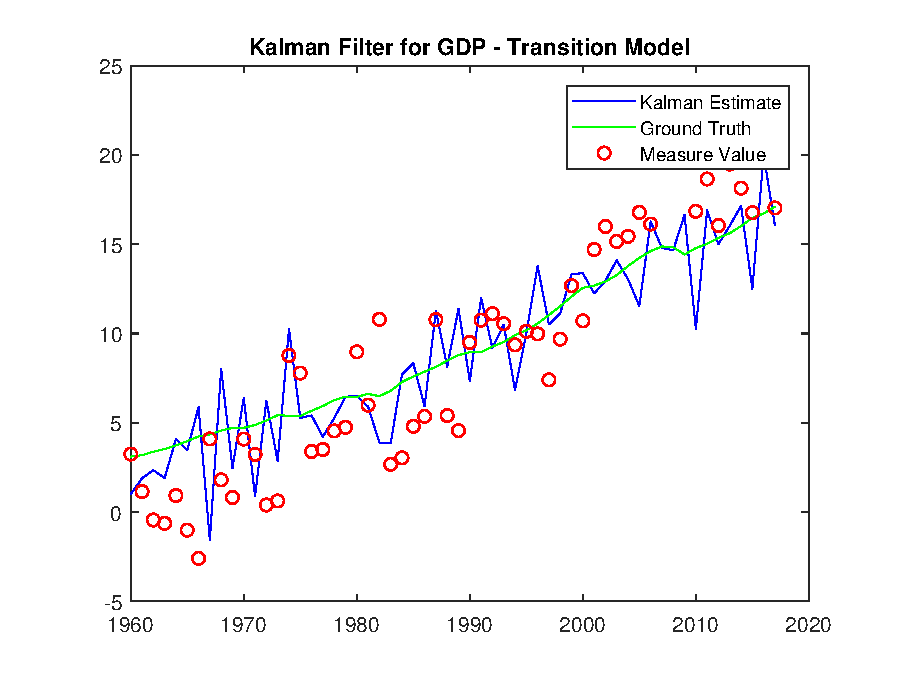
\includegraphics[width=10cm]{kf_2_1}
	
	\caption{Kalman Estimate for GDP (Transition Model Only)}
	\label{fig:kf5}
	
\end{figure}


\subparagraph{GDP Growth Rate Estimate}

The estimate result of GDP growth rate under the transition model is illustrated in figure~\ref{fig:kf6}.

\begin{figure}[htbp]
	
	\centering 
	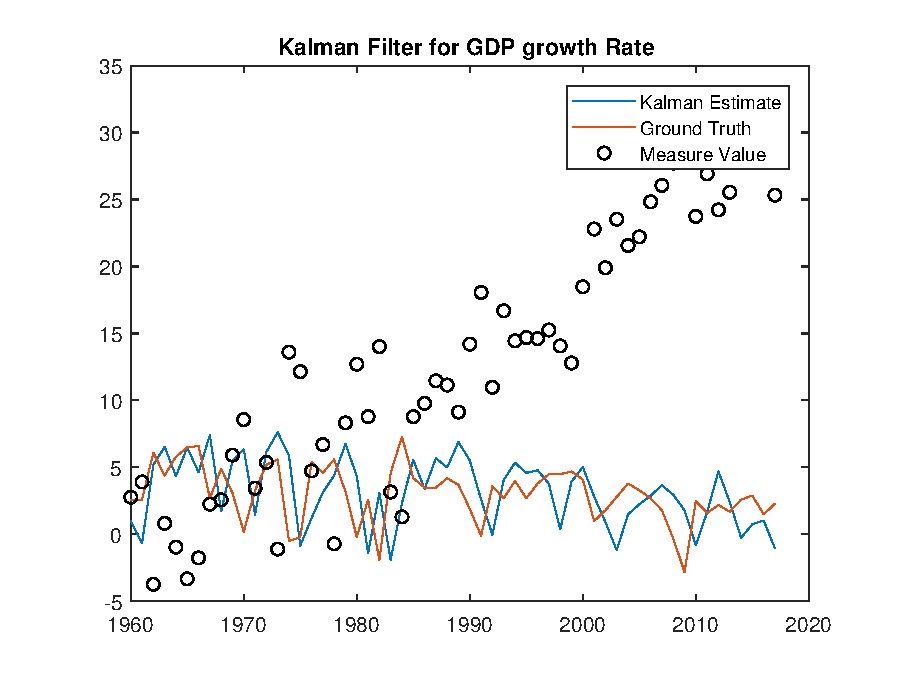
\includegraphics[width=10cm]{kf_2_2}
	
	\caption{Kalman Estimate for GDP Growth Rate (Transition Model Only)}
	\label{fig:kf6}
	
\end{figure}

\paragraph{Estimate Result for The Complete Model}

\subparagraph{GDP Estimate}

The estimate result of GDP under the complete model is illustrated in figure~\ref{fig:kf7}.

\begin{figure}[htbp]
	
	\centering 
	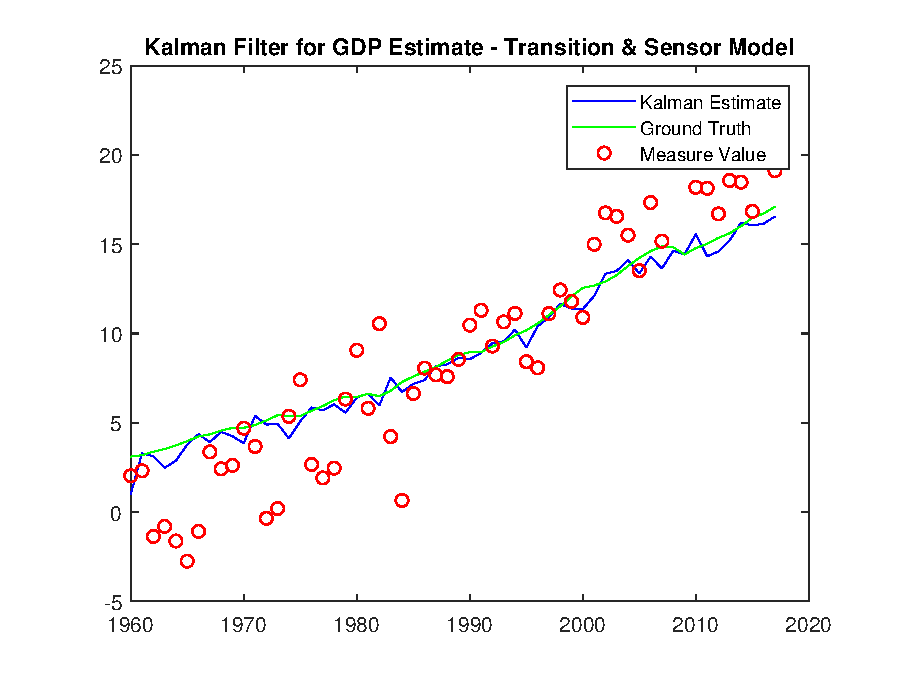
\includegraphics[width=10cm]{kf_2_3}
	
	\caption{Kalman Estimate for GDP Growth Rate (Complete Model)}
	\label{fig:kf7}
	
\end{figure}

\subparagraph{GDP Growth Rate Estimate}

The estimate result of GDP growth rate under the complete model is illustrated in figure~\ref{fig:kf8}.

\begin{figure}[htbp]
	
	\centering 
	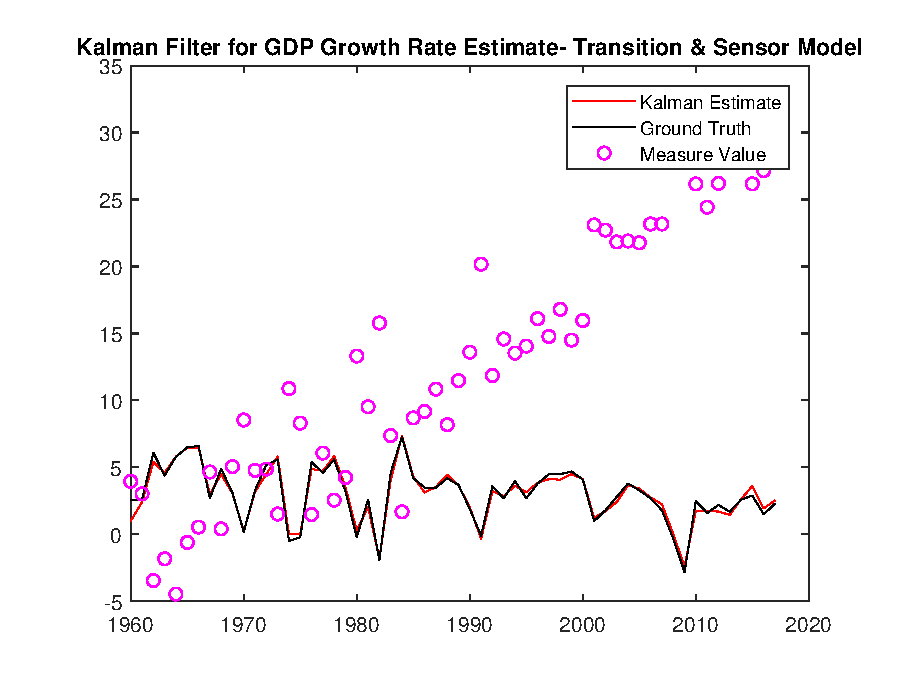
\includegraphics[width=10cm]{kf_2_4}
	
	\caption{Kalman Estimate for GDP Growth Rate (Complete Model)}
	\label{fig:kf8}
	
\end{figure}

\subsection{Discussion}

In the result part, the Kalman estimate result for the sensor model with 2 sensors and 3 sensors are given. 

In this part, the Pearson's coffeicient and the variance of the data to compare the fitting result for the 2 sensors and 3 sensors.

\begin{table}[htbp] 
	\begin{center}
		\caption{Variance of Different Data}
		\begin{tabular}{l|l|l|l}  \hline
			& Category  & Transition Model & Complete Model \\ \hline
		GDP &	\textbf{GDP Ground Variance} & 18.6672 & 18.6672 \\  
			
			& 2 Sensors Fitting Variance &  22.5705  & 19.8861  \\
		&	3 Sensors Fitting Variance & 23.5823 & 18.6355 \\ \hline
			
	GDP Growth	&	\textbf{GDP growth Rate Variance} & 4.3208 & 4.3208 \\
			
		&	2 Sensors Fitting Variance &  9.0279  & 3.5090 \\
		&	3 Sensors Fitting Variance & 7.1595 &  4.1567 \\ \hline
		\end{tabular}
		
		\label{tab:kf_meaning2}
	\end{center}
\end{table}	

The Pearson's coefficient table. The higher value means that the better fitting result.

\begin{table}[htbp] 
	\begin{center}
		\caption{Pearson's Coefficient $\rho$}
		\begin{tabular}{l|l|l|l}  \hline
			& Category & Transition Model & Whole Model \\ \hline
	
	GDP & 2 Sensor Model  & 0.8712   & 0.9745 \\
	    & 3 Sensor Model  & 0.8938  & 0.9932 \\ \hline
	    
	GDP Growth Rate & 2 Sensor Model & 0.2433  & 0.5353  \\
	 & 3 Sensor Model  & 0.2480  & 0.9694  \\ \hline 
	
	
		\end{tabular}
		
		\label{tab:kf_meaning3}
	\end{center}
\end{table}	

From table~\ref{tab:kf_meaning2} and~\ref{tab:kf_meaning3}, the 3 sensor model illustrated a better fitting result, the variance deviation is smaller and the Pearson's coefficieint is higher.

The sensor model for the GDP growth rate improve the accuracy of the estimate of the GDP growth rate efficiently. 


\bibliographystyle{IEEEtran}  
\bibliography{MyRefs} 
%\addcontentsline{toc}{section}{References}





%-------------------------------------------------------------------------------------------------------





\end{document}
